% Stand-alone preview of Person 2's report sections (NOT the submitted report).
% Build from docs/report/:  latexmk -pdf -outdir=build p2_preview.tex
% The final report uses IEEEtran; P3 includes the same section files there (see README_P2.md).
\documentclass[10pt,twocolumn]{article}
\usepackage[margin=0.75in]{geometry}
\usepackage{graphicx,amsmath,url,booktabs}
\usepackage[hidelinks]{hyperref}
\graphicspath{{../diagrams/}{../../results/figures/}}
\title{INFT 6000 HW3 --- Group 4\\\large Preview: Sections 3 and 7.2 (Person 2)}
\author{}\date{}
\begin{document}
\maketitle
% Stand-in labels for sections written by other members (defined in their files).
\makeatletter
\def\ptwostub#1#2{\expandafter\gdef\csname r@#1\endcsname{{#2}{}{}{}{}}}
\ptwostub{sec:architecture}{2}\ptwostub{sec:antientropy}{4}\ptwostub{sec:consensus}{5}\ptwostub{sec:setup}{7.1}
\makeatother
\setcounter{section}{2}
% Section 3 - Consistency Model and Read/Write Paths (Person 2)
% Figures: ../diagrams/write_path.png, read_path.png, quorum_overlap.png
% Citations: refs_p2.bib (to be merged into docs/references.bib)
\section{Consistency Model and Read/Write Paths}\label{sec:consistency}

Cassandra inherits its replication model from Dynamo~\cite{decandia2007dynamo} and its
storage model from Bigtable~\cite{lakshman2010cassandra}. Every partition is stored on
$N = \mathit{RF}$ replicas chosen by the token ring (Section~\ref{sec:architecture}); in our
cluster $N = 3$, so every node holds every row. There is no primary replica and no leader:
\emph{any} node can coordinate any request, and the client chooses, \emph{per statement}, how
many replicas must answer before the coordinator replies. This choice is the
\emph{consistency level} (CL), and it is the main knob that trades latency and availability
for freshness~\cite{cassdoc-dynamo,abadi2012pacelc}.

\subsection{Consistency levels}

Table~\ref{tab:cl} lists the levels. A level is a number of replica \emph{responses} the
coordinator waits for; it never changes how many replicas \emph{receive} a write---the
coordinator always sends a mutation to all $N$ live replicas. QUORUM is
$\lfloor N/2 \rfloor + 1$, i.e.\ 2 for $N = 3$. The \texttt{LOCAL\_}/\texttt{EACH\_} variants
restrict or extend the quorum to data centres and behave like their global counterparts in
our single-DC cluster. If no level is given, \texttt{cqlsh} uses ONE and the Python driver
uses LOCAL\_ONE~\cite{pydriver}; our data-access layer therefore sets the level explicitly
on every prepared statement.

\begin{table}[t]\centering\footnotesize
\caption{Consistency levels for $N = 3$ replicas in one data centre.}\label{tab:cl}
\begin{tabular}{lcl}\hline
Level & Replies & Notes \\ \hline
ANY & 1 & writes only; a stored hint counts \\
ONE / LOCAL\_ONE & 1 & lowest latency, weakest freshness \\
TWO, THREE & 2, 3 & fixed counts \\
QUORUM / LOCAL\_QUORUM & 2 & majority; tolerates one replica down \\
EACH\_QUORUM & 2 per DC & writes; multi-DC only \\
ALL & 3 & fails if any replica is down \\
SERIAL / LOCAL\_SERIAL & 2 & Paxos phase of LWTs (Section~\ref{sec:consensus}) \\ \hline
\end{tabular}
\end{table}

\paragraph{What is (and is not) guaranteed}
By default Cassandra is \emph{eventually consistent}~\cite{vogels2009eventually}: if writes
stop, replicas converge through hints, read repair and anti-entropy repair, but a read at
ONE may return an older value in the meantime. Choosing read and write levels with
$R + W > N$ makes every read set intersect every write set, so a read returns the most
recent \emph{acknowledged} write; this gives read-your-writes and, together with blocking
read repair, monotonic quorum reads~\cite{cassdoc-readrepair}. It does \emph{not} give
linearizability~\cite{herlihy1990linearizability}: concurrent writes to the same cell are
ordered by timestamps, not by agreement, and a failed write is not rolled back.
Linearizable compare-and-set requires lightweight transactions (Paxos,
Section~\ref{sec:consensus}). Session guarantees in the sense of Terry et
al.~\cite{terry1994session} are thus obtained only through the CL choice, not tracked by
the client.

\subsection{Write path}

Fig.~\ref{fig:write-path} follows one write at QUORUM.
(1)~The token-aware driver hashes the partition key with Murmur3 and sends the request
directly to a replica, which becomes the \emph{coordinator}. It assigns the write a
timestamp (our driver generates monotonic client-side microsecond timestamps).
(2)~The coordinator derives the replica set and checks its gossip view: if fewer than $W$
replicas are believed alive it rejects the request at once with \texttt{Unavailable} and
nothing is written.
(3)~Otherwise it sends the mutation to \emph{all} live replicas. Each replica appends the
mutation to its commit log and applies it to the in-memory memtable; memtables are later
flushed to immutable SSTables and merged by compaction~\cite{cassdoc-storage}. With the
default \texttt{commitlog\_sync: periodic} (10\,s) a replica acknowledges before the
commit log is \texttt{fsync}ed, so single-node durability relies on replication.
(4)~The coordinator answers the client as soon as $W$ acknowledgements have arrived; the
latency is therefore governed by the $W$-th fastest replica. Late acknowledgements are
ignored but the write is still applied.
(5)~For a replica that is down, the coordinator stores a \emph{hint} and replays it when
the replica returns (within \texttt{max\_hint\_window}, 3\,h by default). Hints do not count
towards $W$ (except for ANY), so Cassandra does not use Dynamo's ``sloppy quorum'' to
raise write availability~\cite{cassdoc-hints,decandia2007dynamo}.
If $W$ acknowledgements do not arrive within \texttt{write\_request\_timeout} (2\,s) the
client receives \texttt{WriteTimeout}---which means ``unknown'', not ``failed'': replicas that
did apply the mutation keep it, and the value can surface in later reads.

\begin{figure}[t]\centering
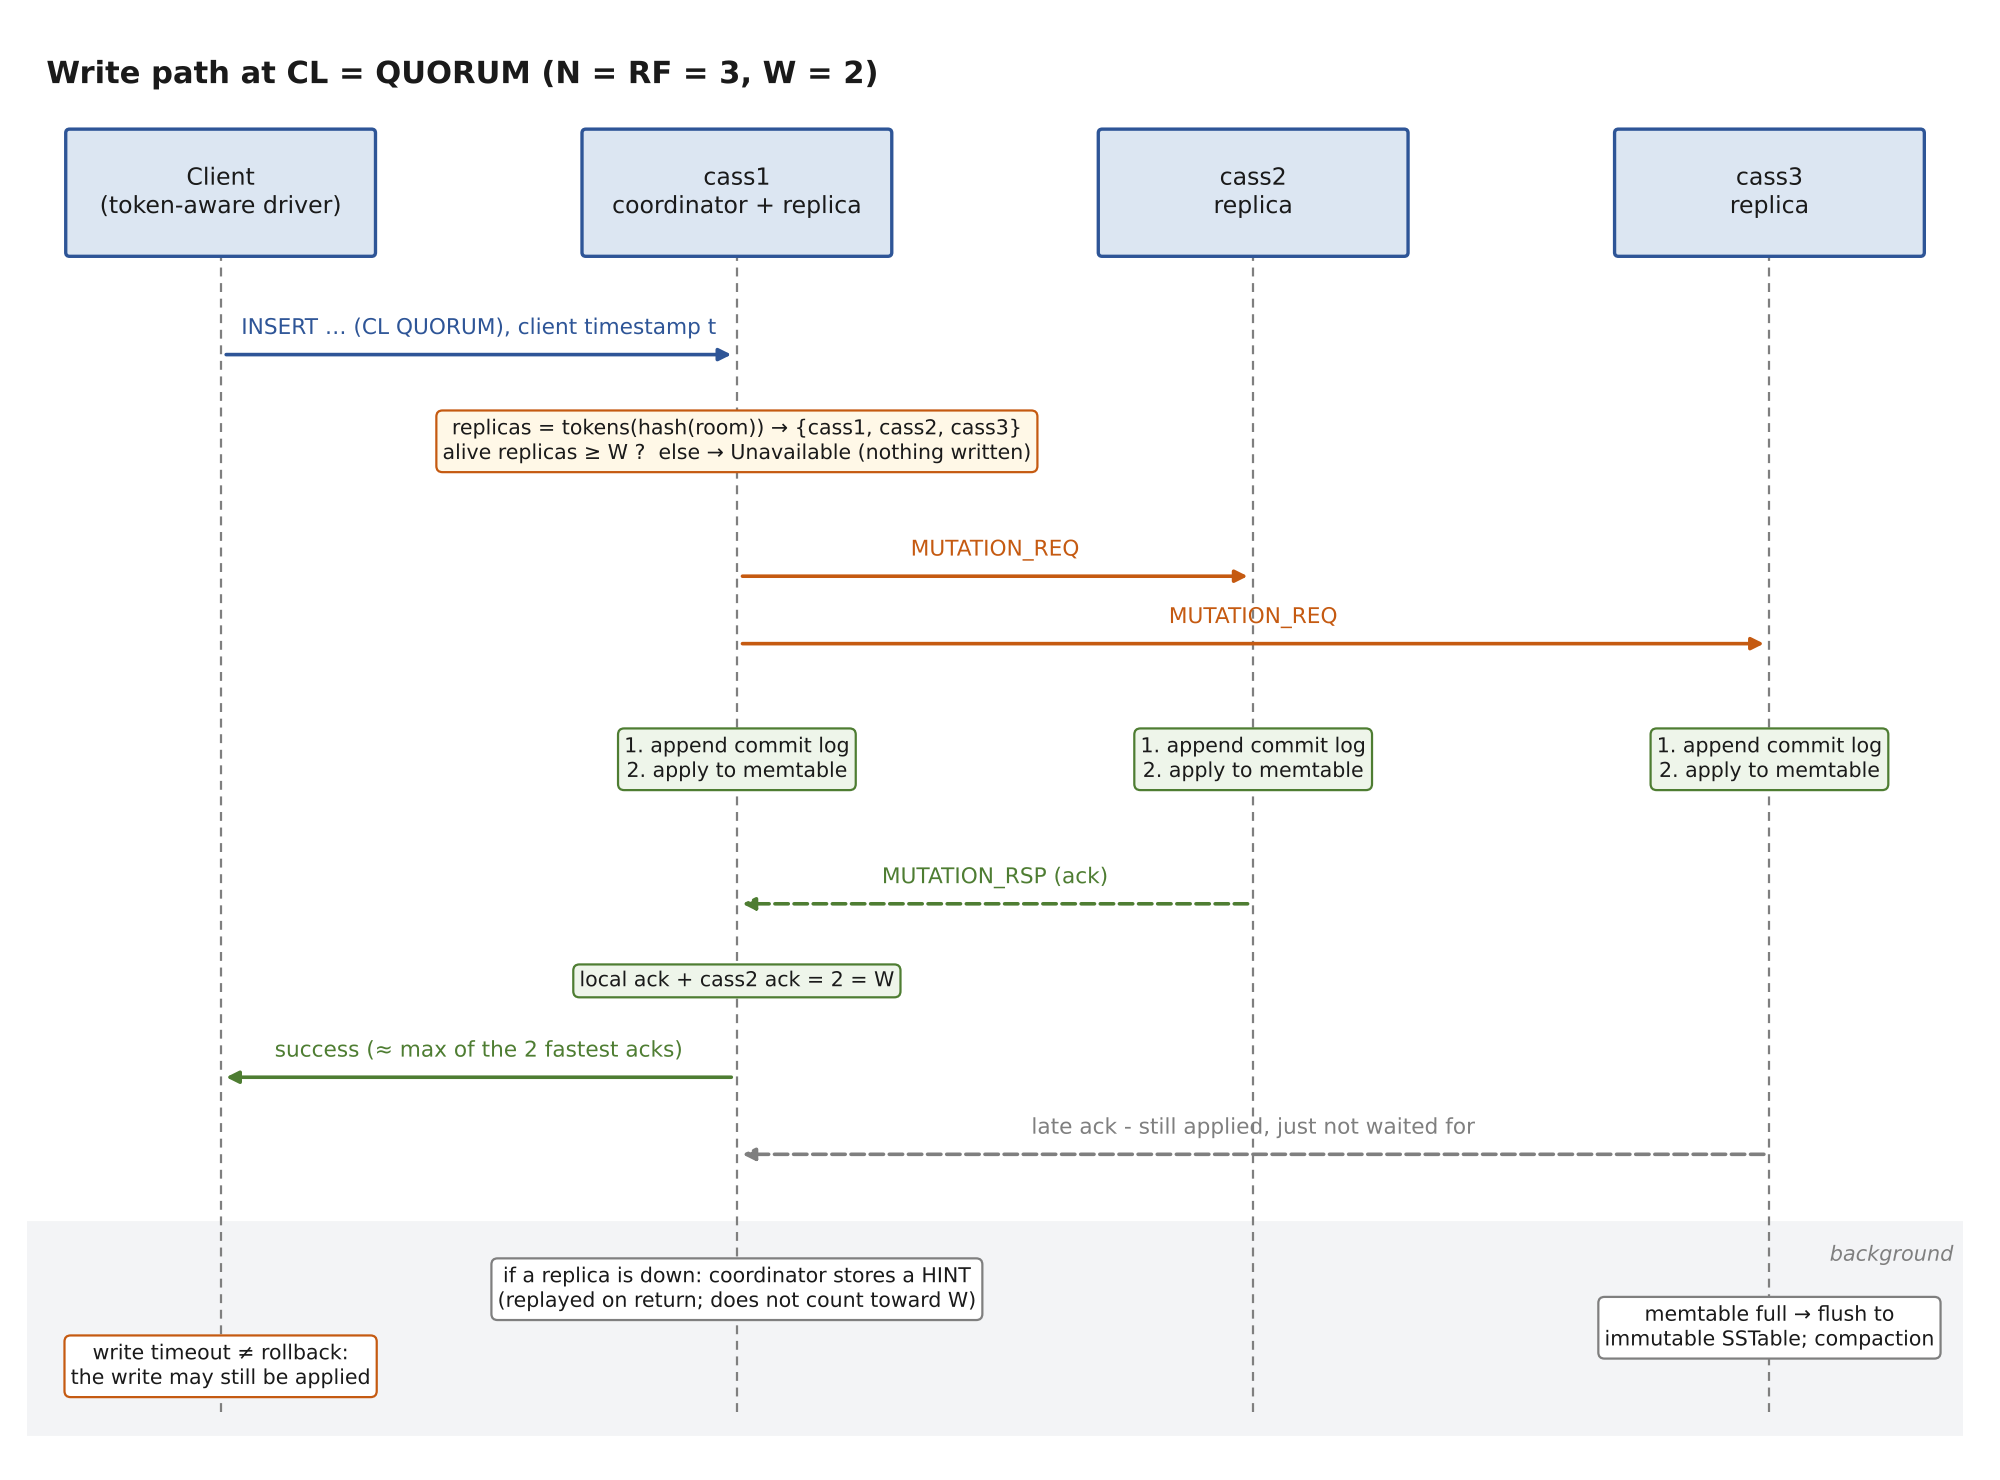
\includegraphics[width=\columnwidth]{write_path.png}
\caption{Write path at QUORUM ($N = 3$, $W = 2$): the coordinator replicates to all three
replicas but replies after two acknowledgements.}\label{fig:write-path}
\end{figure}

\subsection{Read path}

Fig.~\ref{fig:read-path} shows a read at QUORUM.
(1)~The coordinator orders the replicas by the dynamic snitch's latency scores and contacts
$R$ of them: the closest receives a \emph{data} request, the others \emph{digest} requests,
which return only a hash of the result.
(2)~Each replica builds its result by merging the memtable with the SSTables that may
contain the partition (bloom filters and partition indexes avoid the rest).
(3)~If the digests match the data, the coordinator returns it. If they differ, it sends
full-data requests to every replica of the first round, reconciles the responses cell by
cell---the highest timestamp wins (last-write-wins, LWW), with tombstones treated as
timestamped deletions---and
(4)~writes the reconciled value back to the stale replicas it contacted. Since Cassandra 4.0
this \emph{read repair} is \emph{blocking} by default (\texttt{read\_repair = 'BLOCKING'}):
the client receives the result only after the repair mutations are acknowledged, which
guarantees that two successive quorum reads never go backwards in time; the per-table
option \texttt{'NONE'} trades this for lower latency~\cite{cassdoc-readrepair,cass14635}.
At ONE only one replica is read, so there is no digest comparison and no read repair.
(5)~If a replica is slower than the table's 99th-percentile read latency
(\texttt{speculative\_retry = '99p'}), the coordinator sends a redundant request to
another replica to cut the tail. Exp~1 shows this in practice: the traced ONE read
coordinated by cass3 (log \texttt{07\_read\_cass3\_one\_traced.txt}) executed locally and
also logged ``speculating read retry'' towards cass1, which answered with the same row.

Read repair only fixes data that is read, and only on the replicas a read contacts.
Rows that are never read are reconciled by hints or by Merkle-tree anti-entropy repair
(Section~\ref{sec:antientropy}); Exp~4 isolates the three mechanisms.

\begin{figure}[t]\centering
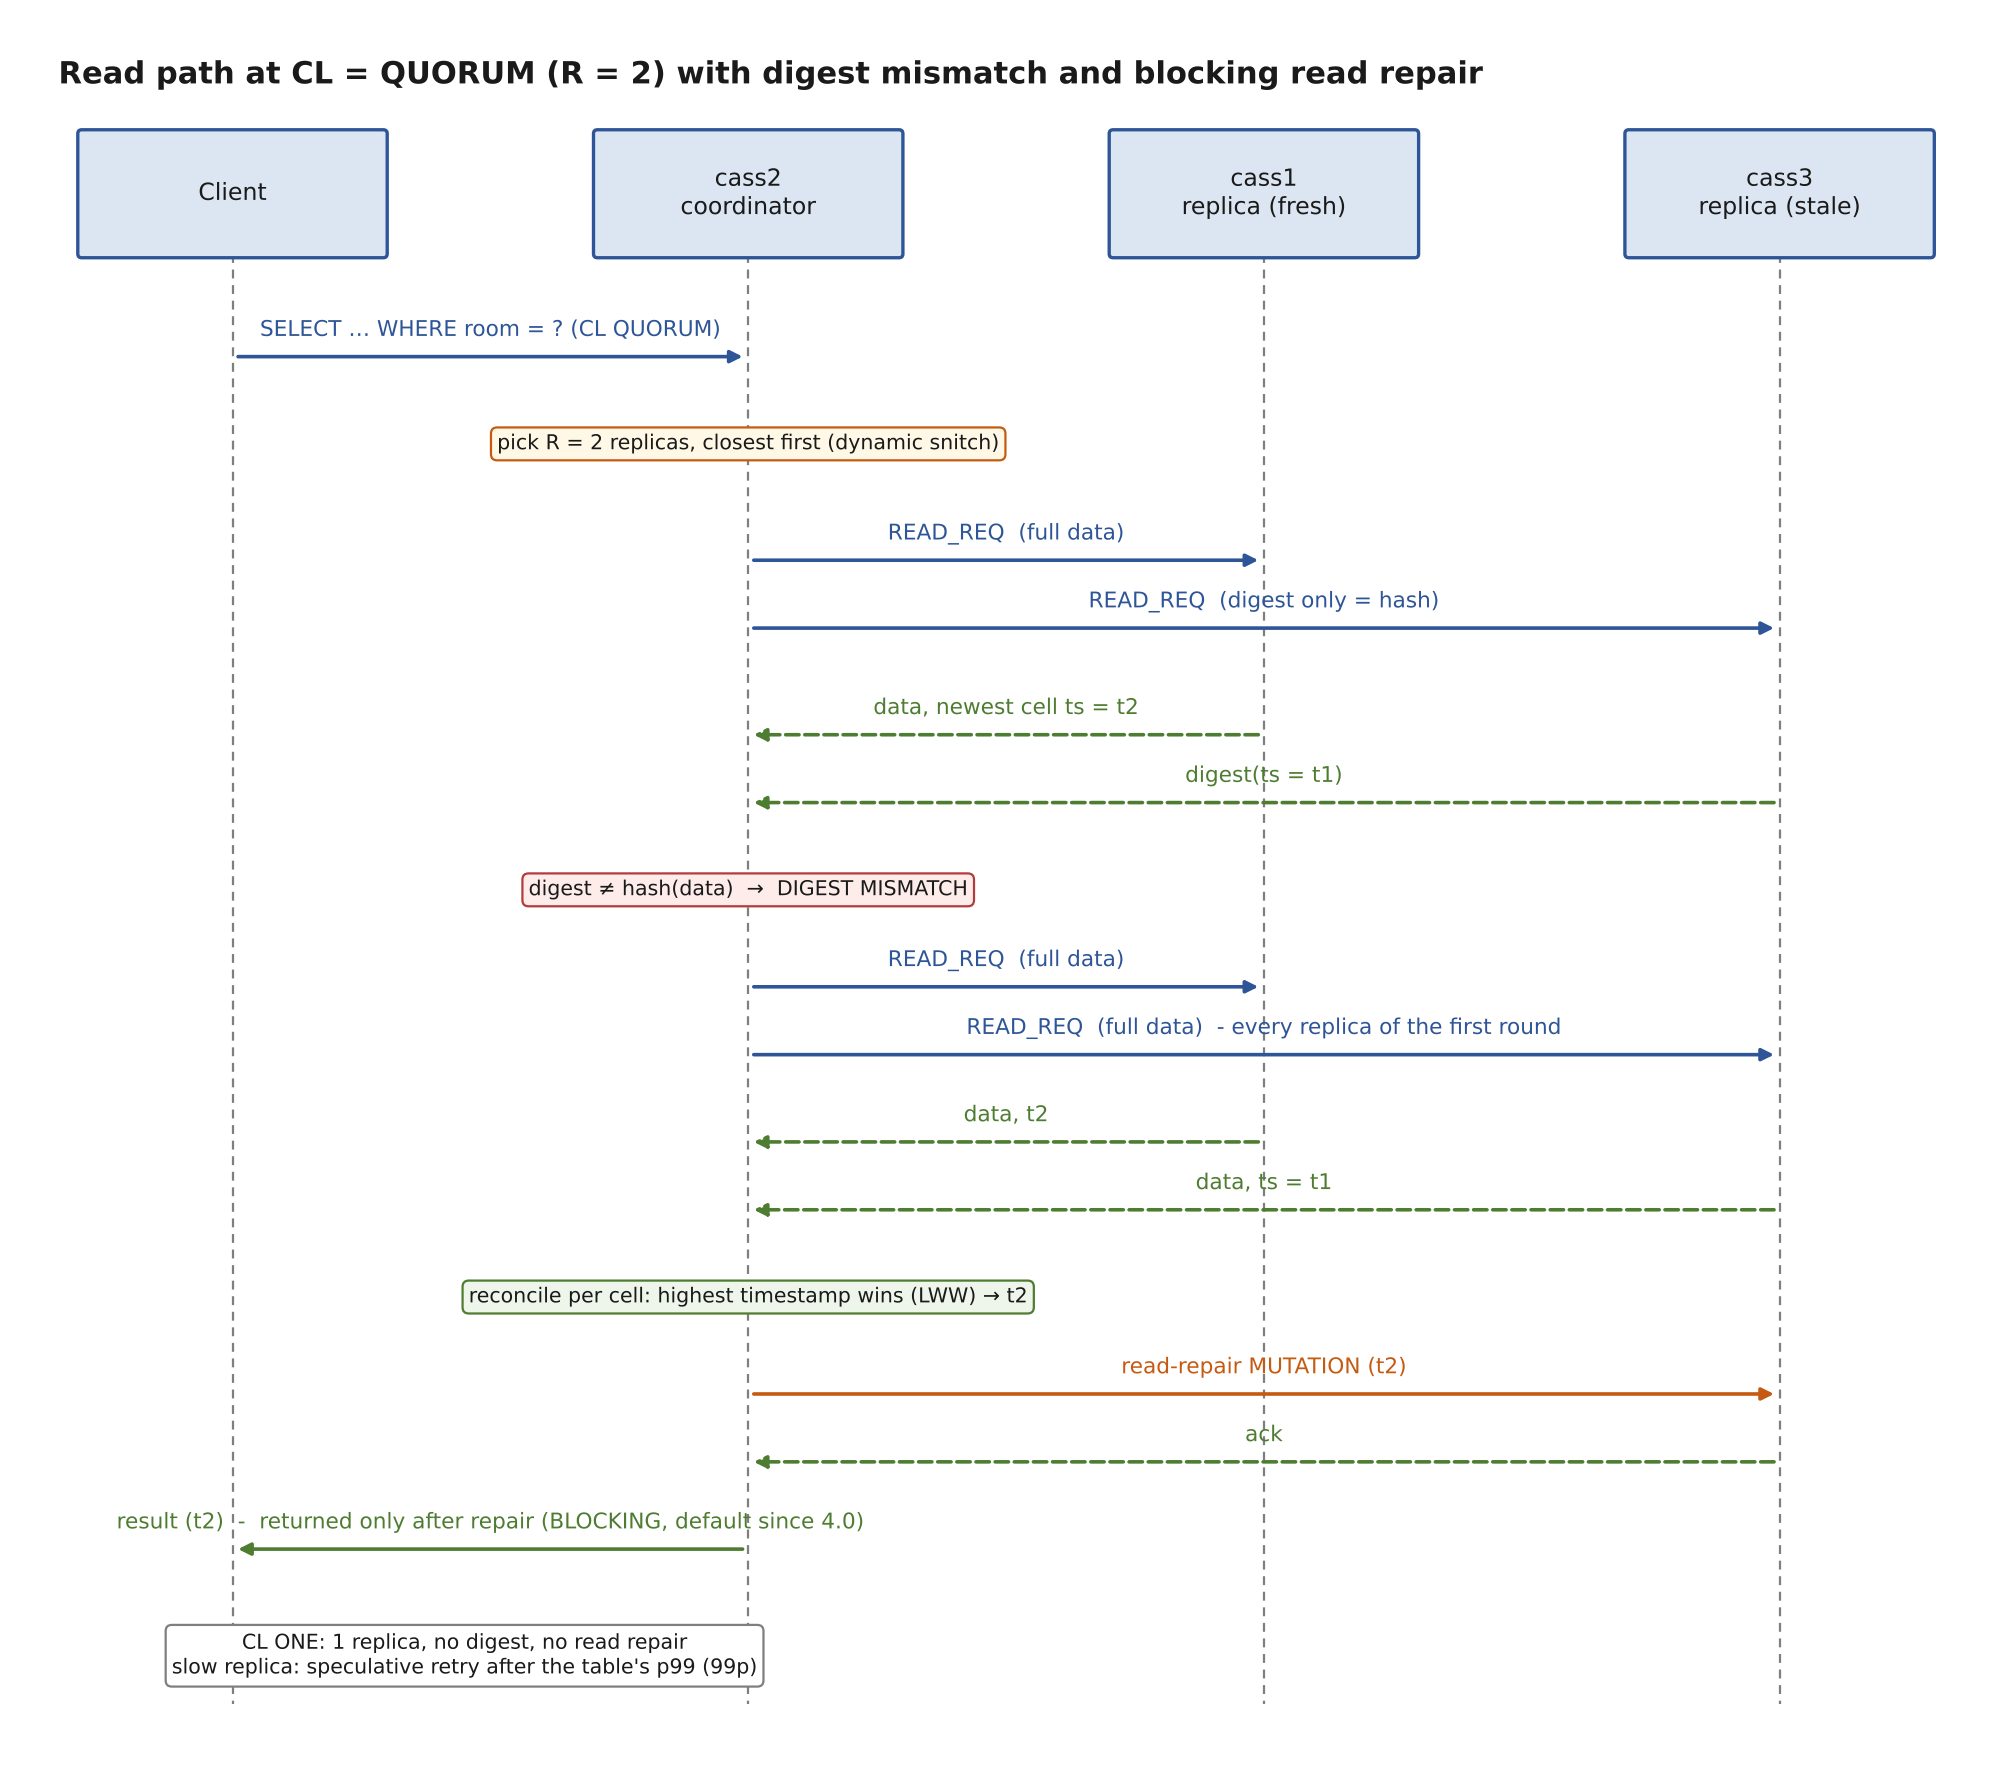
\includegraphics[width=\columnwidth]{read_path.png}
\caption{Read path at QUORUM with a digest mismatch: the stale replica is detected,
reconciled by timestamp and repaired before the client is answered.}\label{fig:read-path}
\end{figure}

\subsection{Quorum mathematics}

With $N$ replicas, writes acknowledged by $W$ and reads served by $R$, the read set and the
write set must share a replica whenever $R + W > N$---the quorum-intersection condition of
weighted voting~\cite{gifford1979weighted}. The shared replica holds the latest acknowledged
value, and timestamp reconciliation makes the coordinator return it.
Table~\ref{tab:quorum} and Fig.~\ref{fig:quorum} give the five pairs measured in Exp~2.
Raising $R + W$ costs availability: a write at $W$ survives $N - W$ failed replicas and a
read at $R$ survives $N - R$, so QUORUM/QUORUM is the only pair that keeps both
operations available with one node down while still overlapping.

\begin{table}[t]\centering\footnotesize
\caption{Quorum arithmetic for $N = 3$ (QUORUM $= 2$).}\label{tab:quorum}
\begin{tabular}{llccl}\hline
$W$ & $R$ & $R+W$ & $R+W>N$ & Failures tolerated \\ \hline
ONE & ONE & 2 & no & writes 2, reads 2 \\
ONE & QUORUM & 3 & no & writes 2, reads 1 \\
QUORUM & QUORUM & 4 & yes & writes 1, reads 1 \\
ALL & ONE & 4 & yes & writes 0, reads 2 \\
ONE & ALL & 4 & yes & writes 2, reads 0 \\ \hline
\end{tabular}
\end{table}

\begin{figure}[t]\centering
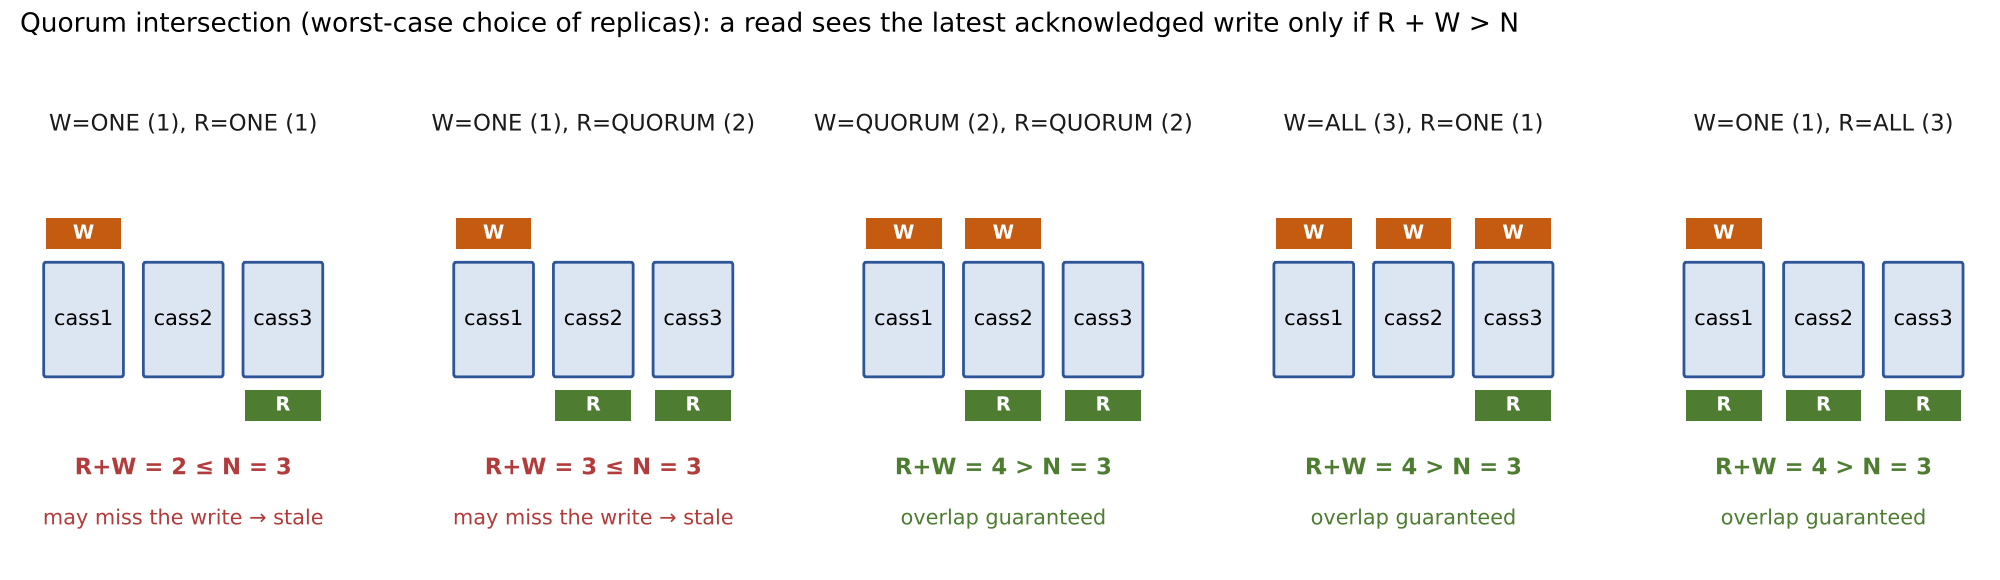
\includegraphics[width=\columnwidth]{quorum_overlap.png}
\caption{Worst-case replica choice for each pair: only pairs with $R + W > N$ always
share a replica with the latest write.}\label{fig:quorum}
\end{figure}

The guarantee rests on four assumptions, and each failure mode is visible in Cassandra.
(i)~\emph{Timestamps order writes.} They come from clocks; with skew, an older write can
carry a higher timestamp and silently win. Our client and all nodes share one host clock,
which removes this effect from our measurements.
(ii)~\emph{Only acknowledged writes count.} A write that timed out may be present on some
replicas; a later read can return it or not, depending on which replicas answer.
(iii)~\emph{No concurrent writer.} Two clients writing the same cell are not serialised;
LWW keeps one value and discards the other without error---Exp~5 shows an acknowledged
write lost this way. $R + W > N$ is therefore a freshness condition, not a correctness
condition for read-modify-write.
(iv)~\emph{Fixed replica set.} During bootstrap or decommission the set of replicas for a
token range changes, and intersection is only maintained by the pending-range logic.

When $R + W \le N$, staleness is \emph{possible}, not certain. Bailis et
al.~\cite{bailis2012pbs} model this as probabilistically bounded staleness: the chance of a
stale read decays quickly with the time since the write, because replicas apply mutations
within milliseconds. Our freshness probe (Section~\ref{sec:results-exp2}) measures the worst
case of this window---a read issued immediately after the acknowledgement, through a
different coordinator.

\subsection{Conflict resolution in brief}

Cassandra does not keep vector clocks or sibling versions as Dynamo
does~\cite{decandia2007dynamo}; each cell carries one timestamp and reconciliation is
deterministic LWW per cell, applied identically during reads, hints, read repair,
anti-entropy and compaction. Two concurrent updates to \emph{different} columns of the same
row are both kept, because merging happens per cell. The cost of this simplicity is that
conflicting updates to the same cell lose data without notice, which is why counters and
LWTs exist as separate mechanisms (Sections~\ref{sec:antientropy} and~\ref{sec:consensus}).

\setcounter{section}{6}
\section{Experimental Results}
\setcounter{subsection}{1}
% Section 7.2 - Results of Experiments 1 and 2 (Person 2)
% Numbers come ONLY from generated/exp2_numbers.tex and generated/exp2_tables.tex, which
% workload/exp2_summary.py writes from results/raw/ (make exp2 && make exp2-report).
% Until then every number prints as a bold "[run make exp2-report]" marker.
\providecommand{\exptwo}[1]{%
  \ifcsname exptwo@#1\endcsname\csname exptwo@#1\endcsname
  \else\textbf{[run make exp2-report]}\fi}
\InputIfFileExists{generated/exp2_numbers.tex}{}{}

\subsection{Results: normal operations and consistency tuning}\label{sec:results-exp2}

\paragraph{Method}
All measurements use the CassChat workload generator (\texttt{workload/runner.py}) in the
client container on the cluster network (Section~\ref{sec:setup}). The data-access layer
routes each request token-aware to a replica, disables driver retries
(\texttt{FallthroughRetryPolicy}) and speculative execution, and uses a 5\,s client timeout,
so every server-side failure is counted rather than hidden. Latency is measured in the
client around each request (\texttt{perf\_counter}) and logged with its outcome and
coordinator, one CSV row per operation. Fixed-rate runs are \emph{open loop}: requests are
scheduled every $1/\text{rate}$ seconds regardless of earlier responses
(200\,ops/s, 8 threads, 60\,s measured after a 10\,s warm-up that is not logged), for
each mode (write, read, mixed 50/50) and CL, repeated \exptwo{reps} times with the CL order
rotated between repetitions. Reads fetch the newest 10 messages of one of 100 rooms
preloaded with 10{,}000 messages. A closed-loop run per CL (32 threads, 30\,s) gives the
saturation throughput. The \emph{freshness probe} writes $\texttt{last\_seq} = n$ through
coordinator $A$ at CL $W$ and, as soon as the write is acknowledged, reads it through a
different coordinator $B$ at CL $R$; the read is stale if it returns less than $n$.

\paragraph{Experiment 1}
The committed Exp~1 evidence (\texttt{results/logs/exp1/}) shows the expected healthy
baseline: three nodes Up/Normal with one schema version and the Murmur3 partitioner; every
node owns 100\,\% of the data effectively; \texttt{getendpoints} lists all three
addresses for partition \texttt{general}; and a row written at QUORUM through cass1 was read
at ONE through cass3. The trace of that read shows the coordinator serving the row
locally and, through speculative retry, also from cass1 (Section~\ref{sec:consistency}).
The 60\,s baseline at QUORUM (mixed, 200\,ops/s) completed \exptwo{exp1-ops} operations
with \exptwo{exp1-err}\,\% errors at \exptwo{exp1-tput}\,ops/s; latency was
p50 \exptwo{exp1-p50}\,ms, p95 \exptwo{exp1-p95}\,ms and p99 \exptwo{exp1-p99}\,ms.

\paragraph{Latency and throughput}
Table~\ref{tab:exp2-grid} and Fig.~\ref{fig:exp2-latency} summarise the grid.
\exptwo{sentence-ordering} \exptwo{sentence-tail} \exptwo{sentence-errors}
\exptwo{sentence-rate} \exptwo{sentence-saturation}

\InputIfFileExists{generated/exp2_tables.tex}{}{%
  \begin{table}[t]\centering\footnotesize
  \caption{Experiment 2 results (generated by \texttt{make exp2-report}).}\label{tab:exp2-grid}
  \textbf{[run make exp2-report]}\end{table}}

\begin{figure}[t]\centering
\IfFileExists{../../results/figures/exp2_latency_percentiles.png}{%
  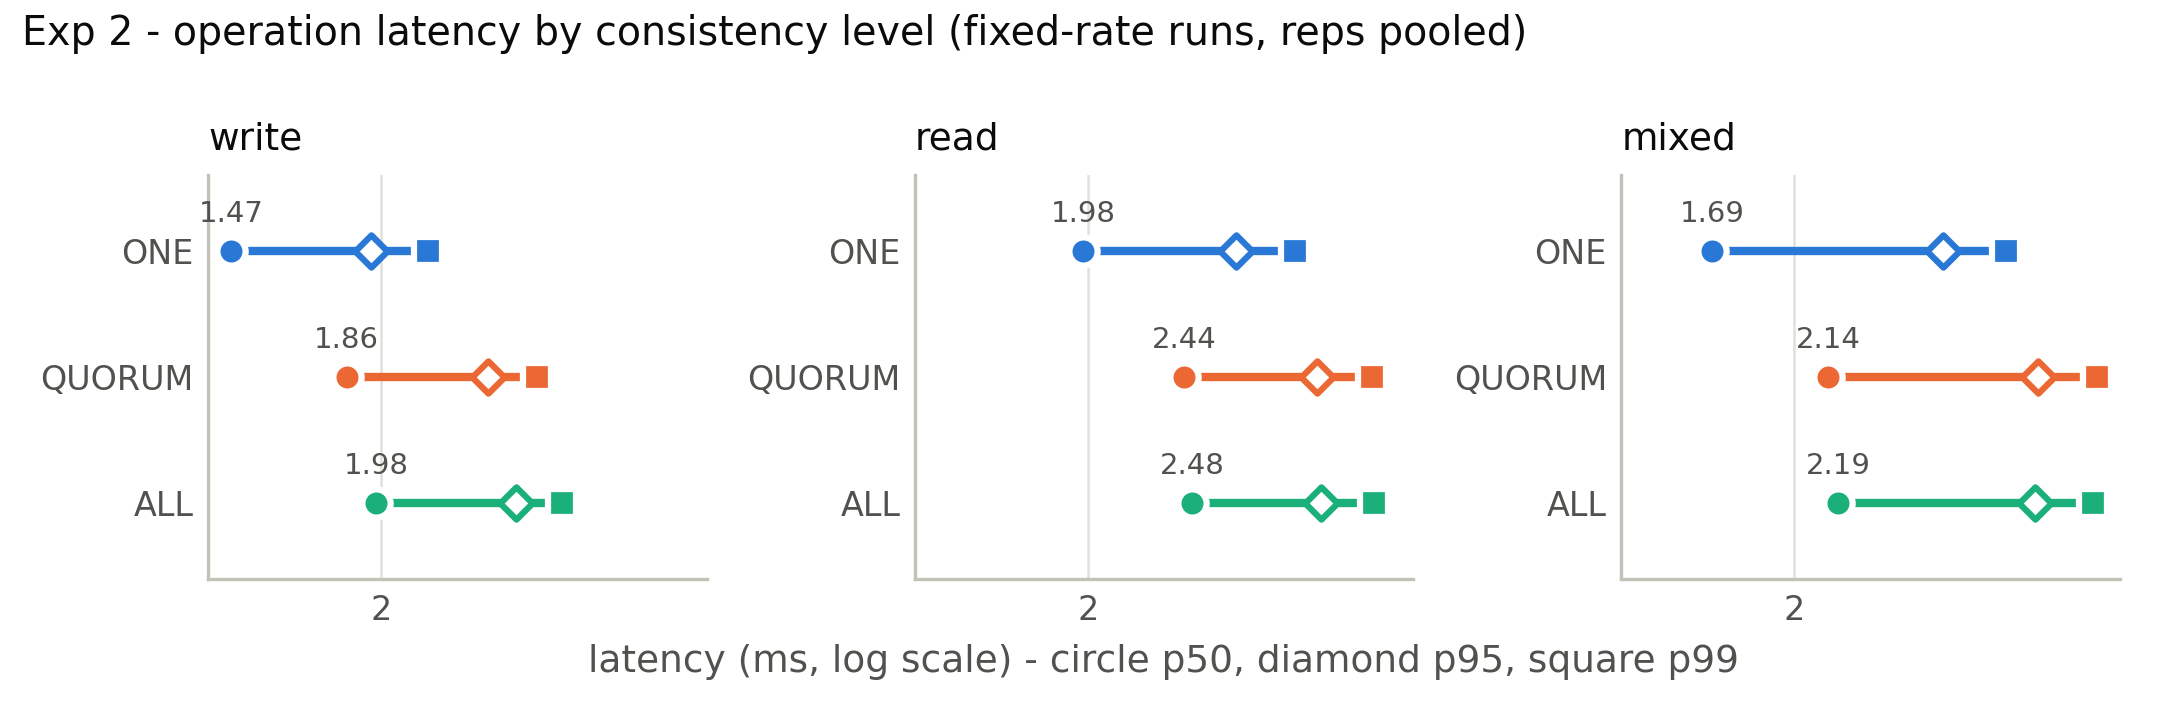
\includegraphics[width=\columnwidth]{exp2_latency_percentiles.png}}{%
  \fbox{\parbox{0.9\columnwidth}{\centering\vspace{8mm}\textbf{[run make exp2-report]}\vspace{8mm}}}}
\caption{Experiment 2: p50 (circle), p95 (diamond) and p99 (square) latency per consistency
level; fixed-rate runs, repetitions pooled.}\label{fig:exp2-latency}
\end{figure}

\paragraph{Freshness}
Table~\ref{tab:exp2-probe} lists the probe results. \exptwo{sentence-staleness}
The probe measures the most demanding case---a read issued within one client round trip of
the acknowledgement---so these rates are an upper bound for the steady-state workload, in
line with the PBS model~\cite{bailis2012pbs}.

\paragraph{Interpretation}
On a healthy cluster the price of a stronger level is latency, not availability: the
coordinator performs the same replication work for every write and only waits longer.
That price is small here because all replicas share one host and the replica round trip is
sub-millisecond; across racks or data centres the gap between ONE and ALL grows with the
slowest replica's distance, which is exactly the latency term of PACELC's ``else'' branch
(EL vs.\ EC)~\cite{abadi2012pacelc}. The \emph{availability} side of the trade-off appears
only when replicas fail: ALL rejects writes as soon as one replica is down, while QUORUM
keeps both reads and writes available and still overlaps (Exp~3 and Exp~5).

\paragraph{Threats to validity}
(i)~All nodes and the client share one machine, so network latency is unrealistically low
and CPU contention between containers can add noise; we recorded \texttt{docker stats}
during every run to rule out saturation. (ii)~The Python client is CPU-bound near
saturation, so closed-loop throughput is a lower bound on cluster capacity. (iii)~With a
bounded number of threads, an open-loop generator falls back to closed-loop behaviour if
all threads are busy; the runner reports operations that started more than 50\,ms late, and
such cells are rerun. (iv)~The working set fits in memtables and the page cache, so reads
rarely touch disk. (v)~The probe can detect staleness only within its own round trip;
a zero count means the inconsistency window was shorter than that, not that it does not
exist. (vi)~Three repetitions give limited statistical power; the table reports the
standard deviation of throughput across repetitions.

\bibliographystyle{ieeetr}
\bibliography{refs_p2}
\end{document}
